% Options for packages loaded elsewhere
\PassOptionsToPackage{unicode}{hyperref}
\PassOptionsToPackage{hyphens}{url}
%
\documentclass[
  parskip,
  openany]{scrreprt}
\author{}
\date{\vspace{-2.5em}}

\usepackage{amsmath,amssymb}
\usepackage{lmodern}
\usepackage{iftex}
\ifPDFTeX
  \usepackage[T1]{fontenc}
  \usepackage[utf8]{inputenc}
  \usepackage{textcomp} % provide euro and other symbols
\else % if luatex or xetex
  \usepackage{unicode-math}
  \defaultfontfeatures{Scale=MatchLowercase}
  \defaultfontfeatures[\rmfamily]{Ligatures=TeX,Scale=1}
\fi
% Use upquote if available, for straight quotes in verbatim environments
\IfFileExists{upquote.sty}{\usepackage{upquote}}{}
\IfFileExists{microtype.sty}{% use microtype if available
  \usepackage[]{microtype}
  \UseMicrotypeSet[protrusion]{basicmath} % disable protrusion for tt fonts
}{}
\makeatletter
\@ifundefined{KOMAClassName}{% if non-KOMA class
  \IfFileExists{parskip.sty}{%
    \usepackage{parskip}
  }{% else
    \setlength{\parindent}{0pt}
    \setlength{\parskip}{6pt plus 2pt minus 1pt}}
}{% if KOMA class
  \KOMAoptions{parskip=half}}
\makeatother
\usepackage{xcolor}
\IfFileExists{xurl.sty}{\usepackage{xurl}}{} % add URL line breaks if available
\IfFileExists{bookmark.sty}{\usepackage{bookmark}}{\usepackage{hyperref}}
\hypersetup{
  hidelinks,
  pdfcreator={LaTeX via pandoc}}
\urlstyle{same} % disable monospaced font for URLs
\usepackage{longtable,booktabs,array}
\usepackage{calc} % for calculating minipage widths
% Correct order of tables after \paragraph or \subparagraph
\usepackage{etoolbox}
\makeatletter
\patchcmd\longtable{\par}{\if@noskipsec\mbox{}\fi\par}{}{}
\makeatother
% Allow footnotes in longtable head/foot
\IfFileExists{footnotehyper.sty}{\usepackage{footnotehyper}}{\usepackage{footnote}}
\makesavenoteenv{longtable}
\usepackage{graphicx}
\makeatletter
\def\maxwidth{\ifdim\Gin@nat@width>\linewidth\linewidth\else\Gin@nat@width\fi}
\def\maxheight{\ifdim\Gin@nat@height>\textheight\textheight\else\Gin@nat@height\fi}
\makeatother
% Scale images if necessary, so that they will not overflow the page
% margins by default, and it is still possible to overwrite the defaults
% using explicit options in \includegraphics[width, height, ...]{}
\setkeys{Gin}{width=\maxwidth,height=\maxheight,keepaspectratio}
% Set default figure placement to htbp
\makeatletter
\def\fps@figure{htbp}
\makeatother
\setlength{\emergencystretch}{3em} % prevent overfull lines
\providecommand{\tightlist}{%
  \setlength{\itemsep}{0pt}\setlength{\parskip}{0pt}}
\setcounter{secnumdepth}{5}
\newlength{\cslhangindent}
\setlength{\cslhangindent}{1.5em}
\newlength{\csllabelwidth}
\setlength{\csllabelwidth}{3em}
\newlength{\cslentryspacingunit} % times entry-spacing
\setlength{\cslentryspacingunit}{\parskip}
\newenvironment{CSLReferences}[2] % #1 hanging-ident, #2 entry spacing
 {% don't indent paragraphs
  \setlength{\parindent}{0pt}
  % turn on hanging indent if param 1 is 1
  \ifodd #1
  \let\oldpar\par
  \def\par{\hangindent=\cslhangindent\oldpar}
  \fi
  % set entry spacing
  \setlength{\parskip}{#2\cslentryspacingunit}
 }%
 {}
\usepackage{calc}
\newcommand{\CSLBlock}[1]{#1\hfill\break}
\newcommand{\CSLLeftMargin}[1]{\parbox[t]{\csllabelwidth}{#1}}
\newcommand{\CSLRightInline}[1]{\parbox[t]{\linewidth - \csllabelwidth}{#1}\break}
\newcommand{\CSLIndent}[1]{\hspace{\cslhangindent}#1}
\usepackage[ ngerman, main=english]{babel}
\usepackage[utf8]{inputenc}
\usepackage[T1]{fontenc}
\usepackage{lmodern}
\usepackage[onehalfspacing]{setspace}
\usepackage[left=1.50cm,right=1.50cm,top=1.50cm,bottom=1.50cm,includehead,includefoot]{geometry}
\usepackage[headsepline]{scrlayer-scrpage}
\usepackage{url}
\usepackage[backend=biber, style=authoryear, giveninits=true, maxbibnames=99, uniquename=init, maxcitenames=2, hyperref=true, date=year]{biblatex}
\usepackage{xpatch}
\usepackage{cleveref}
\usepackage{csquotes}
\usepackage{amsmath}
\usepackage{listings}
\usepackage{booktabs}
\usepackage{longtable}
\usepackage{multirow}
\usepackage{rotating}
\usepackage{subfigure}
\usepackage{graphicx}
\usepackage{float}
\usepackage{acronym}
\usepackage{lipsum}
\usepackage{scrhack}
\emergencystretch=50pt
\clubpenalty = 10000
\widowpenalty = 10000
\displaywidowpenalty = 10000
\automark[section]{chapter}
\renewcommand*{\chaptermarkformat}{}
\renewcommand*{\sectionmarkformat}{}
\setkomafont{title}{\sffamily}
\setkomafont{disposition}{\usekomafont{title}}
\setkomafont{author}{\usekomafont{title}}
\setkomafont{date}{\usekomafont{title}}
\setkomafont{caption}{\sffamily\small}
\setkomafont{captionlabel}{\usekomafont{caption}\bfseries\small}
\setkomafont{pagehead}{\normalfont\scshape}
\ifLuaTeX
  \usepackage{selnolig}  % disable illegal ligatures
\fi

\begin{document}

\begin{titlepage}
\centering
    {\Large Ruprecht-Karls-Universität Heidelberg\\
        Fakultät für Biowissenschaften\\
        Bachelorstudiengang Molekulare Biotechnologie\\}

    {\vspace{\stretch{2}}}
    {\usekomafont{title}

        {\huge Molecular Characterization of Immune Signaling and Metabolic Subtypes in Human Cancer}

        {\Huge }
        
        {\LARGE A Pan-Cancer Analysis with therapeutic outlooks for clear cell renal cell carcinoma}

    }

    \vspace{\stretch{2}}
    {\Large Data Science Project SoSe 2022}

    \vspace{\stretch{2}}

    {\Large
        \begin{tabular}{rl}
            Autoren & Anna von Bachmann, Linda Blaier, Maja Glotz, Tim Wenzel\\
            Heidelberg &18.07.2022\\
        \end{tabular}
    }

    \vspace{\stretch{1}}

\end{titlepage}

\addchap{Abstract}

Characterizing the metabolic and immune landscape in tumors is crucial
to treatment decisions. Based on gene expression data from 9783 patients
we were able to characterize metabolic structures in 33 cancer types and
identified essential alterations in drug metabolism leading to treatment
failure as well as clear distinctions regarding immune signaling. Within
24 of 33 cancer types we were able to define immune signaling subtypes,
highly associated with CD8+ T cell signaling. Going further, we
conducted an analogous analysis for clear cell renal cell cancer and
discovered strong correlations between immune signaling pathways and
immune infiltration. Using immune deconvolution, we got an insight into
the tumor microenvironment of clear cell kidney renal cancer. More
precisely, we were able to characterize the tumor microenvironment
during tumor progression, where an early stage is associated with
macrophage infiltration and progressive CD8+ T cell infiltration.
Further, we compared healthy tissue with tumorous tissue of clear cell
renal kidney cancer, leading to the identification of a neutral and
immune infiltrated subtype, based on CD8+ infiltration. We then
successfully predicted this infiltration rate solely based on two immune
signaling pathways - interleukin 1 and T cell receptor signaling.
Therefore, we created a highly accurate model, to facilitate treatment
decisions, characterizing immune infiltrated subtypes as more
perceivable towards immune therapy. \tableofcontents

\let\cleardoublepage\clearpage
\addchap{List of Abbreviations}

\small

\begin{tabular}{rl}
        ACC & Adrenocortical carcinoma\\
        BLCA & Bladder Urothelial Carcinoma\\
        BRCA & Breast invasive carcinoma\\
        CESC & Cervical squamous cell carcinoma and endocervical adenocarcinoma\\
        CHOL & Cholangiocarcinoma\\
        COAD & Colon adenocarcinoma\\
      DLBC & Lymphoid Neoplasm Diffuse Large B-cell Lymphoma\\
      ESCA & Esophageal carcinoma\\
      FDR & False discovery rate\\ 
      GBM & Glioblastoma multiforme\\
      GSEA & Gene set enrichment analysis\\
      HNSC & Head and Neck squamous cell carcinoma\\
      KEGG & Kyoto encyclopedia of genes and genomes\\
      KICH & Kidney Chromophobe\\
      KIRC & Kidney renal clear cell carcinoma\\
      KIRP & Kidney renal papillary cell carcinoma\\
      LAML & Acute Myeloid Leukemia\\
      LGG    & Brain Lower Grade Glioma\\
      LIHC & Liver hepatocellular carcinoma\\
      LUAD & Lung adenocarcinoma\\
      LUSC & Lung squamous cell carcinoma\\
      MESO & Mesothelioma\\
      OV & Ovarian serous cystadenocarcinoma\\
      PAAD & Pancreatic adenocarcinoma\\
      PC & Principal component\\
      PCA & Principal component analysis\\
      PCPG & Pheochromocytoma and Paraganglioma\\
      PID & Pathway interaction database\\
      PRAD & Prostate adenocarcinoma\\
      RCC & Renal cell carcinoma\\
      READ & Rectum adenocarcinoma\\
      SARC & Sarcoma\\
      SKCM & Skin Cutaneous Melanoma\\
      STAD & Stomach adenocarcinoma\\
      SW & Shapiro-Wilks\\
      TCGA & The cancer genome atlas\\
      TGCT & Testicular Germ Cell Tumors\\
      THCA & Thyroid carcinoma\\
      THYM & Thymoma\\
      TME & Tumor Microenvironment\\
      UCEC & Uterine Corpus Endometrial Carcinoma\\
      UC & Uterine Carcinosarcoma\\
      UMAP & uniform manifold approximation and projection\\
      UVM & Uveal Melanoma\\
        \end{tabular}

\hypertarget{introduction}{%
\chapter{Introduction}\label{introduction}}

Cancer is one of the most prevalent diseases in the world and
responsible for almost 10 million deaths each year (Ferlay \emph{et
al.}, 2021). Therefore, it is a big interest to further understand the
characteristics of cancer in more detail hoping to find new treatment
options. Pan cancer analysis aims to find similarities and differences
across different tumor types. These types of analysis are often based on
The Cancer Genome Atlas (TCGA) which is a comprehensive genome
sequencing database consisting of bulk samples of over 11 000 tumors
from the 33 most prevalent forms of cancer(Cooper \emph{et al.}, 2018).

It is known that cancer cells have certain characteristics that
distinguish them from normal cells, the so-called hallmarks of cancer.
These enable them to evade human protection mechanisms and sustain
uncontrolled cell proliferation. Cancer hallmarks often are a
consequence of altered gene expression patterns (Hanahan and Robert,
2011). Among other things in this project, we want to identify and
compare pathways with altered gene expression who are primarily
responsible for establishing the cancer hallmarks across the 33 tumor
types selected in the TCGA.

The activation of oncogenes and the loss of tumor suppressor gene
functions are the main cause for tumor development. Both can lead to
reprogramming of cellular metabolism. This way cancer cells can cover
their high needs for nutrients even in a nutrient-poor environment. For
example, cancer cells have an increased glucose metabolism due to the
Warburg effect (Warburg \emph{et al.}, 1927; Natalya and Craig, 2016).
Therefore, we also did a pan cancer analysis on metabolic pathways for
which we used pathways curated by the Kyoto Encyclopedia of Genes and
Genomes (KEGG) (Ogata \emph{et al.}, 1999).

Beyond the tumor cells themselves, a tumor type is also characterized by
its microenvironment (TME). Dependent on the composition of immune cells
in the TME, it can either promote or suppress tumorigenesis. To
investigate immune signaling, we used a gene set from the Pathway
interaction database (PID). The respective pathways mainly concern
signaling especially regarding cell cycle and immune response (Schaefer
\emph{et al.}, 2009).

Kidney cancer is one of the most common kinds of cancer. Most kidney
cancer patients are diagnosed with Renal Cell Carcinoma (RCC) of which
renal clear cell carcinoma (KIRC) is the most prevalent form. The
treatment of choice for early stage RCC patients is surgical removal
(Chen \emph{et al.}, 2020). While this is relatively successful with an
overall survival of 60-70\%, the prognosis for late stage RCC is less
than 10\%. This can be attributed to RCC being an intratumorally
heterogenous form of cancer. Additionally, KIRC is resistant to
traditional treatment methods like chemotherapy and radiotherapy
(Dimitrieva \emph{et al.}, 2016). Therefore, novel individualized
treatment options need to be developed (Zhang \emph{et al.}, 2019).

\hypertarget{star-methods}{%
\section{Star Methods}\label{star-methods}}

\hypertarget{uniform-manifold-approximation-and-projection}{%
\subsection{Uniform Manifold Approximation and
Projection}\label{uniform-manifold-approximation-and-projection}}

\texttt{UMAP} is a new developed dimensionality reduction technique
which is very fast and can preserve global structure of data very well.
For that \texttt{UMAP} constructs a high-dimensional graph which is then
used to create a low-dimensional graph to visualize the dataset. The
initial graph is created based on the calculation of Similarity Scores
dependent on the number of nearest neighbors each data point should
have. From that, the low-dimensional representation is created and
iteratively optimized so the structure of the initial dataset is
preserved best which is also done by calculating Similarity Scores
(Leland McInnes, 2018; Becht \emph{et al.}, 2019).

\hypertarget{wilcoxon-rank-sum-and-signed-rank-test}{%
\subsection{Wilcoxon rank-sum and signed-rank
test}\label{wilcoxon-rank-sum-and-signed-rank-test}}

\texttt{Wilcoxon} rank-sum test and \texttt{Wilcoxon} signed-rank test
both are non-parametric statistical hypothesis tests that can be used
when the data does not follow a normal distribution. \texttt{Wilcoxon}
signed-rank test is used to analyze matched-pair or one-sample data. It
tests the null hypothesis that there is no difference in probability
distribution of first and second sample, hence the distribution of
pairwise differences is centered at zero. The test is based on ranked
absolute values of differences (Woolson, 2007). \texttt{Wilcoxon}
rank-sum test is performed when analyzing unpaired-data and is likewise
based on ranked values. The null hypothesis states that there is no
association between the two samples (Rey and Neuhäuser, 2011).

\hypertarget{kruksal-wallis}{%
\subsection{Kruksal-Wallis}\label{kruksal-wallis}}

\texttt{Kruksal-Wallis} test is a rank-based non-parametric hypothesis
test. It is an extension of \texttt{Wilcoxon} rank-sum test and allows
comparing more than two independent datasets. \texttt{Kruksal-Wallis}
test tests the null hypothesis that there is no difference in
distributions of all \(k\) data sets. The alternative hypothesis states
that at least two populations show stochastic heterogeneity (Vargha and
Delaney, 1998; Ostertagová \emph{et al.}, 2014).

\hypertarget{bonferroni-correction}{%
\subsection{Bonferroni correction}\label{bonferroni-correction}}

Multiple statistical testing results in an increased risk for type I
errors (false positives). \texttt{Bonferroni} correction is used to
reduce this type I error rate. For this, the significance level is
adjusted by dividing the \texttt{False\ decovery\ rate} (\texttt{FDR})
by the number of tests (Armstrong, 2014).

\hypertarget{immune-deconvolution}{%
\subsection{Immune deconvolution}\label{immune-deconvolution}}

The immune deconvolution package (Merotto and Sturm, 2022) is used to
obtain immune cell fractions from bulk RNA-sequencing data. The input is
a matrix with genes as rows and samples as columns, containing gene
expression values as transcripts per million (TPM). The deconvolution
algorithm models the expression of a single gene as a linear combination
of the expression of that gene across the different cell types. An
equation for each gene is set up that contains terms of the matrix
multiplication of a signature matrix \(S\) and an immune cell fraction
vector \(F\). The signature matrix \(S\) contains all average gene
expression profiles for each gene in the immune cell types,
respectively. The output using the \texttt{quanTIseq} method is a matrix
containing the immune cell fractions for each sample that have been
re-normalized to sum up to one (Finotello and Trajanoski, 2018).

\hypertarget{gene-set-enrichment-analysis}{%
\subsection{Gene Set Enrichment
Analysis}\label{gene-set-enrichment-analysis}}

Gene set enrichment analysis (\texttt{GSEA}) is algorithm used for
interpretation of gene expression data based on assembly of genes with
similar biological functions, a so called gene set S. \texttt{GSEA}
compares gene expression data between two different phenotypic groups.
Based on these phenotypic labels a ranked list of genes using a ranking
metric is computed, with the goal of identifying gene sets that are not
randomly distributed among the ranked gene list. For this purpose, 3
main steps are performed. Firstly, the Enrichment Score (\texttt{ES}) is
calculated using random walk: Whenever a gene of the gene set is present
in the ranked gene list, the running-sum increases. Whenever, this is
not the case, the running-sum decreases. Increase and decrease are
weighted upon the rank of each gene. The \texttt{ES(S)} of the gene set
is equal to the maximum difference from zero. Secondly,
\texttt{Kolmogorov-Smirnov}test is used to compare the distribution of
the genes in a gene set to the distribution of genes not included in the
gene set. Additionally, the input data is permuted, creating a null
distribution of ES. By comparing the observed \texttt{ES(S)} to the null
distribution, the \(p-value\) is determined. Observed \texttt{ES(S)} and
null distribution are normalized by diving by each mean. For this
purpose, positive and negatives scores are treated separately. Lastly,
an adjustment for multiple hypothesis testing is added. Therefore,
\texttt{Benjamini-Hochberg} (\texttt{BH}) correction is used.
\texttt{BH} correction ranks the \(p-values\) of the ES in increasing
order and then calculated a correction factor by dividing the rank of
the \(p-value\) by the number of tests performed and the
\texttt{false\ discovery\ rate} (\texttt{FDR}). Only is both correction
factor and p-value are smaller than a self-imposed cutoff, the
corresponding \texttt{ES} can be considered significant(Subramanian
\emph{et al.}, 2005).

\hypertarget{binary-logistic-regression}{%
\subsection{Binary logistic
regression}\label{binary-logistic-regression}}

Binary logistic regression is a statistical method used to predict a
dichotomous dependent variable from one or several independent
predictors. In contrast to linear regression, logistic regression does
not require a linear relationship between the independent and the
dependent variable.\\
A logistic regression model is created by training on one dataset and
testing it on another independent one. First, the observations of the
dependent variable of the training dataset are converted into \(0\) an
\(1\) for each outcome, respectively. These data points can be plotted
into a coordinate system and subsequently be moved to positive and
negative infinity through a \(log(odds)\)-transformation. The odds ratio
is calculated using the logit function
\(log(odds)=log(\frac{p}{1-p})\).\\
A regression line is now fitted to these data points and these are
projected onto the fitted line and thus get a new \(log(odds)\)-value.
In order to plot the sigmoidal logistic graph, the new \(log(odds)\)
value of each data point is inserted into the logistic function, which
can be derived by rearranging the \(log(odds)\)-equation
\(p=\frac{e^{log(odds)}}{1+e^{log(odds)}}\).\\
The result of the function is the probability between \(0\) and \(1\)
for each data point to have a \(1\) as the outcome of the dependent
variable. The best fitting linear regression line can be found using the
``maximum likelihood'' that is computed with the probabilities of each
point. The calculation of the likelihood is made for all possible
regression lines, by rotating the line minimally for every new
computation. The best fitting line is the one with the maximum value of
the likelihood.\\
For the evaluation of the regression model \(R^2\)-values and
statistical tests can be considered. Since the residuals cannot be used
to compute \(R^2\) in logistic regression, several pseudo-\(R^2\), such
as the ``McFadden's'' were introduced, which compare the maximum
likelihood of the model to a null model. A Wald-test and a \(chi2\)-test
can be performed to test for the significance of each coefficient and of
the overall model (Peng \emph{et al.}, 2002; Sperandei, 2014).

\hypertarget{materials-and-methods}{%
\chapter{Materials and Methods}\label{materials-and-methods}}

\hypertarget{data-cleaning}{%
\section{Data cleaning}\label{data-cleaning}}

The analysis was focused on two data sets containing bulk-cell
sequencing data. Pan-cancer analysis was performed on gene expression
data of 9783 patients of 33 tumor types (\texttt{DF1}). Focused analysis
was based on gene expression data of normal and tumor tissue of 72 KIRC
patients (\texttt{DF2}). The data obtained was already normalized by
\(log2\)(TPM).\\
Both data sets were filtered for protein-coding genes using
\texttt{biomaRt} package. This reduced gene expression data in
\texttt{DF1} from 60 498 to 19 624 genes and in \texttt{DF2} from 19 624
to 19 186 genes. In \texttt{DF1}, variance was computed for each gene
over all samples and the lower p50-quantile was subsequently removed.
Furthermore, constantly expressed genes only were removed in
\texttt{DF2}, resulting in gene expression data of 18 645 genes.

\hypertarget{tcga-pan-cancer-analysis}{%
\section{TCGA pan-cancer analysis}\label{tcga-pan-cancer-analysis}}

After the data cleaning, as described above, the pan-cancer analysis was
performed on \texttt{DF1}. The dimension reduction methods \texttt{PCA}
and \texttt{UMAP} were used to visualize patients from all tumor types
in a two-dimensional space. For further analysis, hallmarks, KEGG and
PID gene sets were currated from the Molecular Signature
Database(Liberzon \emph{et al.}, 2015) In order to determine the
activity of these genesets in each patient, \texttt{GSEA} was carried
out for each tumor type, respectively. Genes were ranked according to
the \(z\)-score after \(z\)-normalization of each gene across all
samples within every tumor type according to (Peng \emph{et al.}, 2018).
Pathways with an adjusted \(FDR\) \(>0.05\) using
\texttt{Benjamini\ \&\ Hochberg} correction method were considered as
non-significant and their \texttt{NES} was set to zero. Pathway activity
matrices that contained these \texttt{NES} were generated for all gene
sets and could be depicted in heatmaps. Starting from these matrices,
\texttt{hierarchical\ clustering} was performed to find groups of tumor
types with similar regulation. The variance of the\texttt{NES} for each
pathway across all tumor types was computed in order to identify the top
30 pathways with the highest variance and hence most differences in
regulation between tumors. Results of the \texttt{GSEA} with PID
pathways were analyzed in more detail by
\texttt{hierarchical\ clustering} of patients based on the \texttt{NES}
of PID pathways within each tumor type. Significantly different enriched
pathways between the resulting clusters were identified using
\texttt{Kruksal-Wallis} test (\(FDR\): \(5\%\)) and \texttt{Bonferroni}
correction.\\
For all KIRC patients of \texttt{DF1} the immune cell fractions of the
bulk samples were estimated using the \texttt{ìmmunedeconv} package. The
\texttt{quanTIseq} method was used and therefore normalized gene
expression values were transformed back into TPM.

\hypertarget{focused-analysis-identifying-subtypes-in-kirc}{%
\section{Focused Analysis: Identifying subtypes in
KIRC}\label{focused-analysis-identifying-subtypes-in-kirc}}

For focused analysis, KIRC was examined in more detail. The analysis was
based on \texttt{DF2}. Data cleaning was performed as described above.\\
First, differential gene expression in tumor tissue compared to normal
tissue was analyzed by calculation of the Fold change
\(FC =(mean condition 1) / (mean condition 2)\) for each gene, where
condition one represents gene expression of tumor tissue and condition
two gene expression of normal tissue. Statistical significance was
determined using \texttt{Wilcoxon} signed-rank test with
\texttt{Bonferroni} correction, as \texttt{Shapiro-Wilks} test indicated
no normality of the data.\\
The second part of this analysis was focused on differential pathway
activity. Pathway activity matrices were determined using \texttt{GSEA},
where genes were ranked based on their Fold change. Pathways with an
adjusted \(p\)-value \(>0.05\) were considered as non-significant, hence
their \texttt{NES} was set to zero. Hallmark pathways, KEGG pathways and
PID pathways were analyzed. For PID and KEGG pathways, patients were
clustered based on their pathway activity. Subclusters of patients were
visualized for each gene set by \texttt{UMAP} calculated on
\texttt{PCA}-results and subsequently identified by \texttt{k-means}
clustering. Optimal number of clusters was determined using
\texttt{elbow} method and \texttt{silhouette} method. Pathways that were
crucial for this clustering and were significantly different between
those clusters were detected by \texttt{Wilcoxon} rank-sum test for two
clusters and \texttt{Kruksal-Wallis} test for three clusters, both with
\texttt{Bonferroni} correction.

\hypertarget{predicting-immune-infiltration-with-logistic-regression}{%
\section{Predicting immune infiltration with logistic
regression}\label{predicting-immune-infiltration-with-logistic-regression}}

A binary logistic regression model was created based on the pathway
activity of KIRC samples from \texttt{DF1} and tested on \texttt{DF2}.
The dependent variable to be predicted was the ``Immune infiltration''
of samples. The independent variables were pathways chosen from the most
differentially significantly expressed PID pathways between the three
clusters that have emerged in the PID clustering of KIRC patients in
\texttt{DF1}. All patients of the cluster with highest pathway activity
were marked as immune infiltrated with a ``\(1\)'' and all other
patients with a ``\(0\).'' The logistic regression was performed to
predict the immune infiltration in the samples of \texttt{DF2}. The
performance was eventually evaluated with statistical tests and an
ROC-curve with computation of the AUC-value.

\hypertarget{packages}{%
\section{Packages}\label{packages}}

The analysis was performed using Rversion 4.2.0 and Rstudio. Packages
that have been used are listed in Appendix (see Table 6.1)

\hypertarget{results}{%
\chapter{Results}\label{results}}

\hypertarget{tcga-pan-cancer-analysis-1}{%
\section{TCGA pan-cancer analysis}\label{tcga-pan-cancer-analysis-1}}

\hypertarget{gsea-deciphers-differences-in-immune-and-metabolic-signaling-across-tumor-types}{%
\subsection{GSEA deciphers differences in immune and metabolic signaling
across tumor
types}\label{gsea-deciphers-differences-in-immune-and-metabolic-signaling-across-tumor-types}}

\begin{figure}[h]
 \begin{center}
   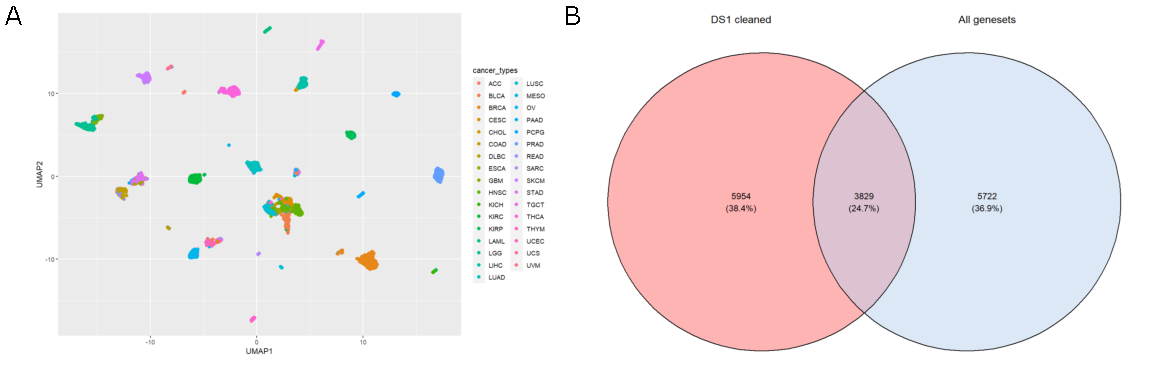
\includegraphics{~/Desktop/GitHub/2022-topic-02-team-02/09_figures/Panel0_Ebene 1.pdf}
  \end{center}
  \caption{\textbf{Clustering of 33 tumor types based on gene expression} (A) `UMAP` besed on gene expression levels show clustering between different tumor types (B) Venn-diagram shows overlap between the significantly differentially expressed genes and genes in the gene sets Hallmark, KEGG and PID}
  \label{UMAP}
\end{figure}

Visualizing the 33 tumor types based on gene expression using
\texttt{PCA} and \texttt{UMAP} revealed that gene expression landscape
is highly diverse. Nontheless, tumor types, which all differ severely in
their phenotype and histopathology, appear to form clusters upon gene
expression (see \Cref{UMAP} \(A\)). To asses the foundation of these
clusters, we utilized several gene sets, including hallmark, PID and
KEGG, which include \texttt{24,7\%} of our highly differentially
expressed genes and were used for further analysis using \texttt{GSEA}
(see \Cref{UMAP} \(B\)).

\begin{figure}[h]
 \begin{center}
   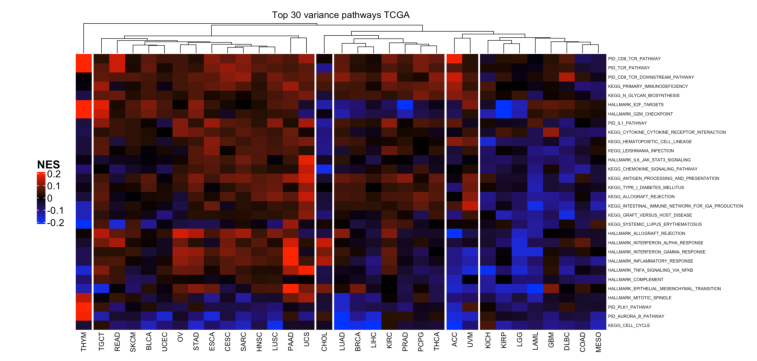
\includegraphics{~/Desktop/GitHub/2022-topic-02-team-02/09_figures/Panel6_v2_Ebene 1.pdf}
  \end{center}
  \caption{\textbf{GSEAresults for 33 tumor types} Heatmap showing top 30 variant gene sets}
  \label{hm}
\end{figure}

\texttt{GSEA} was performed on \texttt{DF1} showing diverse pathway
patterns across tumor types. In order to visualize the enrichment
results, heatmaps of the pathway activity matrices were plotted. Four
main clusters of the 33 tumor types could be identified in the hallmark
\texttt{GSEA}. In general, many pathways did not show a remarkable
enrichment across all tumor types. Strikingly, immune response
associated pathways, like Interferon and Interleukin singaling, were
significantly upregulated in PAAD, OV and STAD and downregulated in LGG,
UVM and ACC. Moreover, pathways promoting cell proliferation like E2F
and G2M-checkpoint were exceptionally upregulated in TGCT and THYM and
downregulated in KIRP, PRAD and LGG (see \Cref{hmap} \(A\)).\\
The heatmap based on KEGG \texttt{GSEA} results showed four clusters as
well (see \Cref{hmap} \(B\)). Noticeably, O-glycan biosynthesis was
highly upregulated in every single tumor type, while pathways for
one-carbon metabolism, homologous recombination and cell cycle were
downregulated. The cluster with UVM, SARC, SKCM, ACC and PCPG showed
high positive enrichment in metabolic pathways, like carbohydrate and
drug metabolism. Pathways associated with antigen presentation and
autoimmune responses were significantly downregulated in the cluster
with DLBC, LAML and KICH, as well as in CHOL and upregulated in almost
all other tumor types.\\
Based on the top 30 pathways according to their variance, several
clusters across tumor types could be resolved (see \Cref{hm}). The
pathways included immune-, metabolic- and hallmark-associated pathways.
The highest variance overall was computed for CD8 TCR, TCR and CD8 TCR
downstream pathways. Interferon, interleukin and complement signaling
pathways were often either up- or downregulated together in tumor types.
An exceptional regulation signature could be seen in THYM, where TCR-
and cell-cycle-related pathways were highly upregulated. CHOL showed a
unique pattern as well with high \texttt{NES} in interferon- and
inflammatory- response gene sets.

\hypertarget{identification-of-immune-signaling-subtypes-in-24-tumor-types}{%
\subsection{Identification of immune signaling subtypes in 24 tumor
types}\label{identification-of-immune-signaling-subtypes-in-24-tumor-types}}

\begin{figure}[h]
  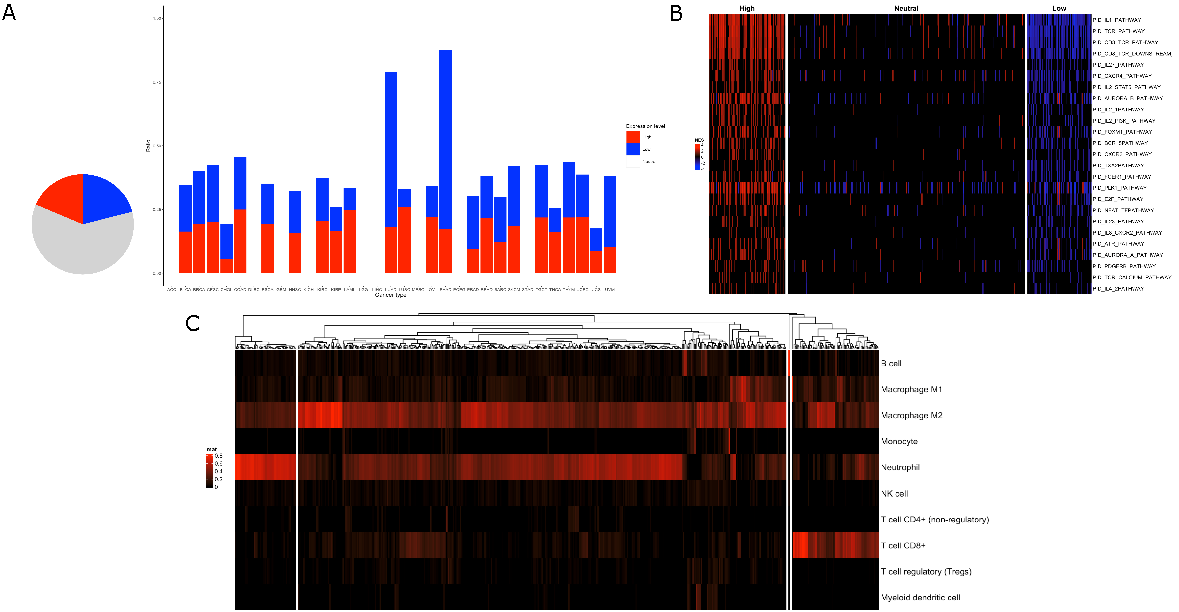
\includegraphics{~/Desktop/GitHub/2022-topic-02-team-02/09_figures/Panel3_Ebene 1.pdf}
  \caption{\textbf{Immune signaling subtypes identified in 24 tumor types and association with immune infiltration in KIRC} (A) Ratio of "High", "Low" and "Neutral" immune signaling expression over all patients and per tumor type (B) Heatmap showing exemplary results of clustering for KIRC (C) Heatmap showing immune infiltration in KIRC}
  \label{pengplot}
\end{figure}

In addition to pathway activity patterns that differ between the 33
tumor types, we next focused on assessing heterogeneity within each
tumor type. For this purpose, we used PID signaling pathways to detect
whether subtypes form based on our \texttt{GSEA} results. Hence, we
identified three subtypes, ``upregulated,'' ``downregulated'' and
``neutral'' in 24 out of 33 tumor types using
\texttt{hierarchical\ clustering} (see \Cref{pengplot} \(A\)).
Significant pathways were filtered using \texttt{Kruksal-Wallis} test
with an \(FDR < 0.05\) and \texttt{Bonferroni} correction. Those
subtypes are only relative within one cancer type and are not
representative compared to normal tissue. The ``neutral'' subtype is the
most common in 22 of 24 tumor types, the only exception being LUAD and
PAAD, which are dominated by the ``downregulated'' subtype. Generally,
the ``neutral'' subtype is present in more than 50\% of the cancer
patients upon the 24 tumor types characterized by successful subtyping.
The ``downregulated'' and ``upregulated'' subtype however are
approximately equally distributed. The subtypes were particularly
distinguished by CD8+ T cell receptor signaling in all 24 tumor types.

In \Cref{pengplot} \(B\) an exemplary result of the subtype
identification is shown for the cancer type KIRC, where the ``neutral''
subtype is predominant. The top 20 pathways ranked according to their
\(p-value\) are displayed. The differently expressed pathways with the
highest significance are Interleukin 1 and Interleukin 27 pathways, as
well as pathways related to T cell specific receptor signaling. Beyond
immune signaling pathways, cell cycle regulatory pathways including E2F,
a transcription factor associated with cell proliferation, and Aurora B,
which plays a role in mitosis, appear to differ between the 3 subtypes
(Yang and Sladek, 1995). Therefore, the subtype with the most
immune-cell related expression patterns shows the highest upregulation
in cell cycle promoting pathways, characterizing this subtype as high
proliferating. An analogous correlation appears in the ``downregulated''
and ``neutral'' subtype.

Based on PID pathway activities, we conducted a more in-depth analysis
of the TME in KIRC. Therefore, we performed immune deconvolution to
assess the total amount of immune cells present in tumor tissue (see
\Cref{pengplot} \(C\)). Patients in the ``upregulated'' subtype could be
mapped to high CD8+ T-cell infiltration, whereas macrophages M2 and
neutrophiles showed lower infiltration compared to the other two
subtypes. Nonetheless, it is visible that other types of immune cells
are outstandingly present in the TMEs of the ``neutral'' and
``downregulated'' subtype. The latter subtype showed highest
infiltration rates in neutrophils, whereas the ``neutral'' subtype is
characterized by high macrophage, as well as medium neutrophile
infiltration. Other immune cells such as NK cells and B cells were not
detectable upon all subtypes. Consequently, the subtypes differ not in
immune infiltration in general, as the pathways expression patterns
suggest, but are characterized by the presence of different immune cell
types.

\hypertarget{focused-analysis-on-kirc}{%
\section{Focused analysis on KIRC}\label{focused-analysis-on-kirc}}

\hypertarget{characterization-of-metabolic-and-immune-signaling-landscape-in-kirc}{%
\subsection{Characterization of metabolic and immune signaling landscape
in
KIRC}\label{characterization-of-metabolic-and-immune-signaling-landscape-in-kirc}}

\begin{figure}[h]
 \begin{center}
   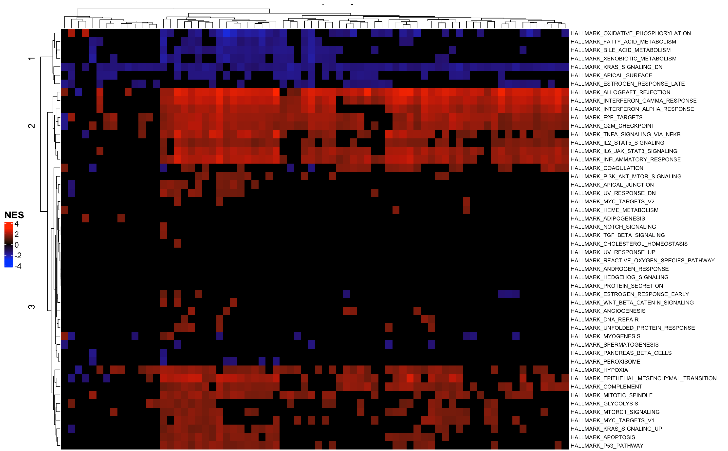
\includegraphics{~/Desktop/GitHub/2022-topic-02-team-02/09_figures/Panel4_v2_Ebene 1.pdf}
  \end{center}
  \caption{\textbf{Identification of differences between healthy and tumorous tissue in KIRC } Heatmap showing differentially expressed hallmark pathways}
  \label{volcano}
\end{figure}

After characterizing differences within KIRC patients, we next wanted to
identity differentially expressed genes and pathways between tumorous
and healthy tissue. Using the binary logarithm of the mean Fold change
between both tissue types, we encountered that the tumorous tissue
features both up and down regulated genes (see \Cref{volcanoap} \(A\)).
To further analyze which parameters are crucial in distinguishing
tumorous from healthy tissue, we used \texttt{GSEA} on 3 gene sets: PID,
KEGG, and Hallmark.

The most frequently enriched pathways, which showed differential
expression in at least 50 of 72 patients, were mapped to allograft
rejection, interferon gamma response and cell cycle regulators, such as
E2F, G2M and KRAS. Consequently, both immune response and cell cycle
regulators appear to play an important role in tumor development and
hence occur in the majority of KIRC patients. Noticeably, all oncogenes
besides the KRAS pathway are upregulated (see \Cref{volcanoap} \(B\)).

\hypertarget{cancer-hallmark-pathways-form-subclusters-in-kirc}{%
\subsubsection{Cancer hallmark pathways form subclusters in
KIRC}\label{cancer-hallmark-pathways-form-subclusters-in-kirc}}

To characterize subtypes within the 72 KIRC patients, we next looked at
each gene set individually. We categorized the hallmark pathways into
three subclusters, where certain pathways are either upregulated,
downregulated or not significantly differentially expressed at all (see
\Cref{volcano} \(C\)). The downregulated subtype was mainly mapped to
fatty acid metabolism, whereas the upregulated subtype consists of cell
cycle regulatory pathways as well as immune signaling pathways.
Nonetheless, the expression patterns within these 3 subtypes of hallmark
gene sets are not homogenously distributed upon all KIRC patients. Using
\texttt{hierarchical\ clustering}, two clusters could be identified, one
smaller cluster, which shows expression levels close two zero, and one
bigger cluster with highly fluctuating expression patterns.

\hypertarget{identification-of-two-kirc-subtypes-that-differ-in-pathways-related-to-immune-signaling-and-cell-cycle-regulators}{%
\subsection{Identification of two KIRC subtypes that differ in pathways
related to immune signaling and cell cycle
regulators}\label{identification-of-two-kirc-subtypes-that-differ-in-pathways-related-to-immune-signaling-and-cell-cycle-regulators}}

\begin{figure}[h]
  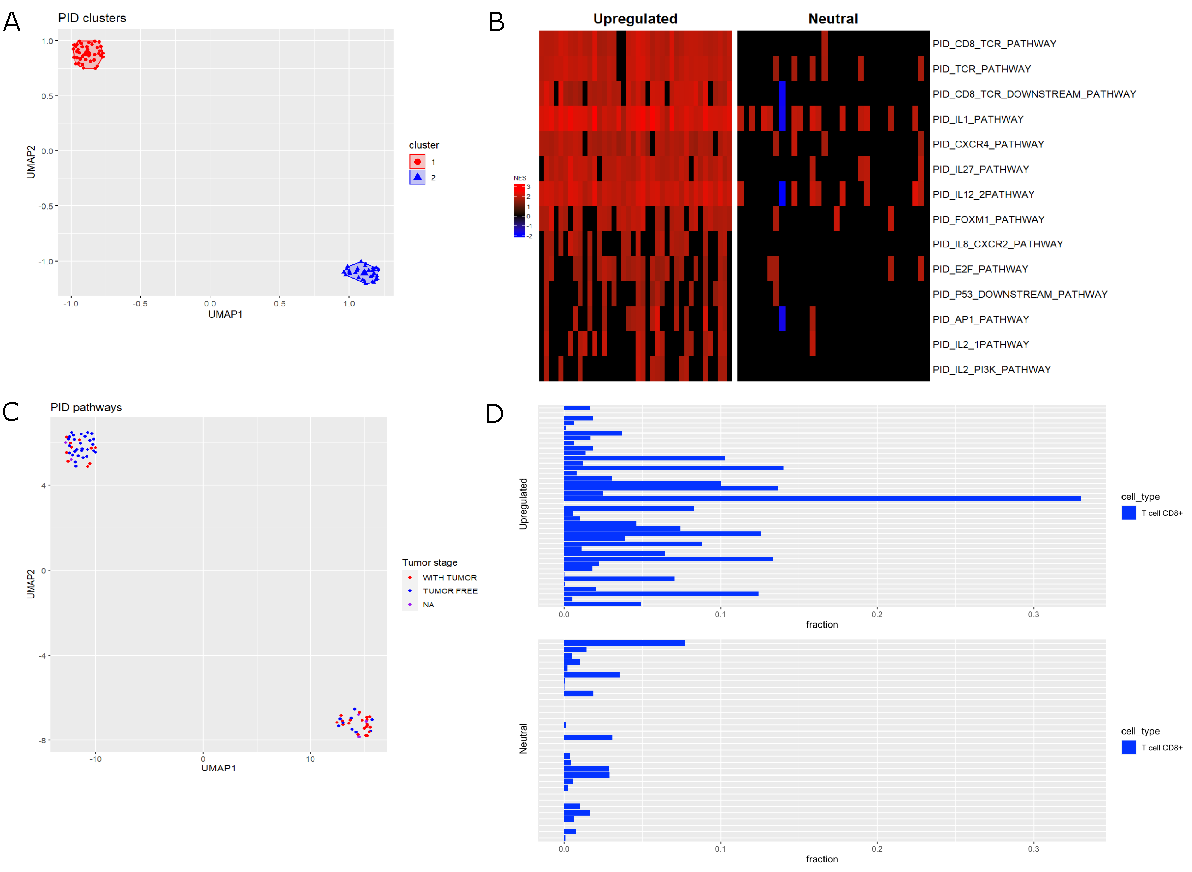
\includegraphics{~/Desktop/GitHub/2022-topic-02-team-02/09_figures/Panel1_Ebene 1.pdf}
  \caption{\textbf{Identifying Immune subtypes within KIRC }(A) k-means clustering of KIRC based on PID pathways (B) Heatmap showing differentially expressed pathways between both clusters (C) Proportion of "Tumor free" patients within each PID cluster (D) Fractions of CD8+ infiltration within each PID cluster}
  \label{pid}
\end{figure}

To determine signaling pathways that distinguish KIRC tumor tissue from
normal tissue, PID pathways were analyzed in more detail. \texttt{GSEA}
revealed that significantly enriched pathways are mainly upregulated and
indicated sample subclusters (see \Cref{tuk} \(A\)). \texttt{k-means}
clustering based on \texttt{UMAP} allowed identification of two distinct
clusters (see \Cref{pid} \(A\)).Next, \texttt{Wilcoxon} ranked-sum test
with \texttt{Bonferroni} correction determined 14 pathways that
significantly differ between the two clusters, hence are crucial for
formation of these two clusters.\Cref{pid} \(B\) shows distinct
differences in \texttt{NES} scores of these pathways in both clusters
and indicate an ``upregulated'' and ``neutral'' subtype. These
differences include pathways that play an important role in cell cycle
regulation, such as E2F and P53 pathway (Polager and Ginsberg, 2009).
Noticeably, a majority of significantly differently pathways are related
to immune response as interleukin pathways (e.g.~IL1, IL2) or T cell
specific receptor signaling. More precisely, top significant pathways
refer to CD8+ T cells, thus potentially differential numbers of these
cells between both clusters. This lead was confirmed by immune
deconvolution, where the ``upregulated'' subtype is associated with
higher CD8+ T cell fractions (see \Cref{pid} \(D\)). Consequently, the
``upregulated'' cluster shows higher CD8+ T cell infiltration compared
to the ``neutral'' subtype characterizing two different TMEs.\\
Additional patient data was provided, such as gender and tumor stage and
was examined with regard to PID clusters. Only a correlation between PID
subtypes and tumor stage could be observed, as \(70.0\%\) of patients in
the ``upregulated'' cluster are tumor free, while in the ``neutral''
cluster, only \(28.1\%\) of patients characterize as tumor free (see
\Cref{pid} \(C\)).

\hypertarget{immune-infiltration-subtypes-can-be-projected-to-kegg-signaling-and-metabolic-pathways}{%
\subsubsection{Immune infiltration subtypes can be projected to KEGG
signaling and metabolic
pathways}\label{immune-infiltration-subtypes-can-be-projected-to-kegg-signaling-and-metabolic-pathways}}

\begin{figure}[h]
  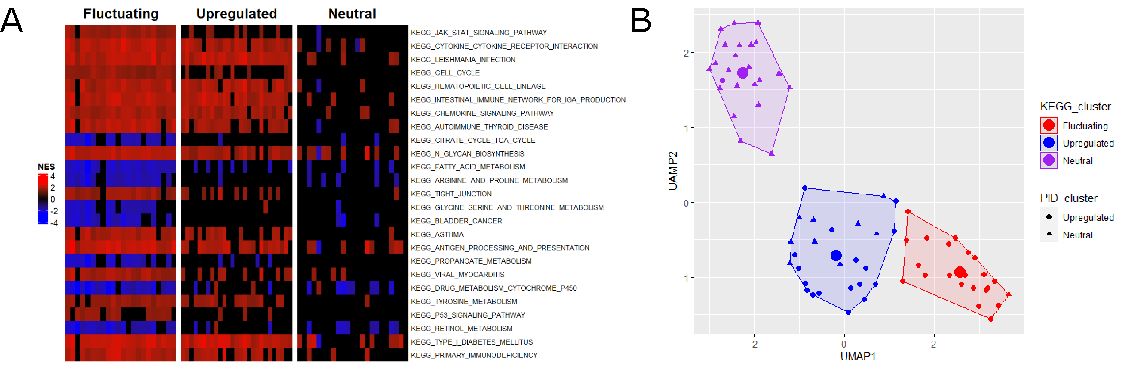
\includegraphics{~/Desktop/GitHub/2022-topic-02-team-02/09_figures/Panel2_Ebene 1.pdf}
  \caption{\textbf{Identifying Metabolic and Signaling subtypes within KIRC} (A) k-means clustering based on KEGG pathways (B) Mapping of PID clusters onto KEGG clusters}
  \label{kegg}
\end{figure}

Next, KEGG pathways were investigated more precisely. \texttt{GSEA}
shows that enriched KEGG pathways in tumor compared to normal tissue
were both, up- and downregulated (see \Cref{tuk} \(B\)). Based on
\texttt{UMAP}, patients could be divided into three subtypes by
\texttt{k-means} clustering. Pathways, that are significantly different
between clusters, were determined using \texttt{Kruksal-Wallis} test
with \texttt{Bonferroni} correction. This allowed identification of a
``fluctuating'' cluster showing both up- and downregulation, one
``upregulated'' cluster with high or neutral \texttt{NES} and one
``neutral'' cluster mainly without pathway enrichment (see \Cref{kegg}
\(A\)). KEGG pathways, that are upregulated in the ``fluctuating'' and
``upregulated'' subtypes, but not the in ``neutral'' subtype, include
pathways that are mainly associated with immunological processes but
also cell cycle. In this context, immunological processes refer to
disease related pathways, such as diabetes mellitus, as well as cytokine
and chemokine signaling and antigen processing and presentation.\\
Moreover, pathways that are downregulated in the ``fluctuating'' subtype
but neutral in both other subtypes relate mostly to metabolic pathways,
such as fatty acid, amino acid, and drug metabolism, as well as TCA
cycle. Moreover, KEGG clusters show similar subdivision of samples as
PID clusters. In \Cref{kegg} \(B\) it can be seen that the
``fluctuating'' KEGG cluster mainly matches patients of the
``upregulated'' PID cluster, while the ``neutral'' KEGG subtype includes
mostly patients of the ``neutral'' PID subtype. Additionally, the
``upregulated'' KEGG cluster corresponds to both PID clusters.

\hypertarget{binary-logistic-regression-model-to-predict-immune-infiltration-based-on-pathway-activity}{%
\section{Binary logistic regression model to predict immune infiltration
based on pathway
activity}\label{binary-logistic-regression-model-to-predict-immune-infiltration-based-on-pathway-activity}}

The binary logistic regression model predicts immune infiltration in
patients based on the pathway activity (\texttt{NES}) of
\texttt{PID\_TCR\_PATHWAY} and \texttt{PID\_IL1\_PATHWAY}. Both
independent variables significantly contribute to the model as can be
seen in Table \Cref{tab}, which depicts the model properties.

\begin{table}[ht]
  \begin{center}
 \begin{tabular}{ |p{4.5cm}||p{3cm}|p{3cm}|p{3cm}|  }
  \hline
  \multicolumn{4}{|c|}{Logistic regression model results} \\
  \hline
   & \textbf{Estimate} & \textbf{Standard error} & \textbf{p-value}\\
  \hline
  Intercept   &  $-2.5856$  & $0.2059$ &   $<2e-16$\\
  PID\_TCR\_PATHWAY &   $0.9727$  & $0.2027$   & $1.59e-06$\\
  PID\_IL1\_PATHWAY & $1.1651$ & $0.1934$ &  $1.70e-09$\\
 \hline
 \end{tabular}
 \end{center}
 \label{tab}
\end{table}

\begin{figure}[ht]
  \scalebox{.5}{\input{~/Desktop/GitHub/2022-topic-02-team-02/09_figures/Panel7_version3_Ebene 1.pdf}}
  \caption{Logistic regression for prediction of immune infiltration (A) Regression model for $PID\_TCR\_PATHWAY$ and $PID\_IL1\_PATHWAY$ (B) Confusion Table (C) ROC-curve for model performance}
  \label{log}
\end{figure}

By taking the exponent of the coefficients in Table \Cref{tab}, the
returned value implies that for every increase of \(1\) in \texttt{NES}
of the TCR and the IL-1 pathway, the odds-ratio for a patient being
immune infiltrated increases by the factor \(2.64517\)(\(164.5\%\)) and
\(3.206149\) (\(220.6\%\)), respectively. The logistic function plots of
each independent variable show that a higher enrichment score indicates
a higher probability of a patient being classified as ``Immune
infiltrated'' (see \Cref{log} \(A\)). The contribution of each
coefficient to the model was evaluated and confirmed with a
\texttt{Wald’s} test, where both TCR (\(p= 1.590e-06\)) and IL-1 pathway
(\(p= 1.701e-09\)) were significant. The significance of the whole model
in contrast to a null-model was confirmed by McFadden's pseudo-\(R^2\)
(\(R_{Mc}^2=0.5074508\)) and the p-value of the overall
\texttt{chi-square} statistic (\(p=7.860549e-60\)).\\
The model was tested on KIRC patients in \texttt{DF2} and classified
\(42\) out of \(72\) patients with a probability threshold of
\(p > 0.5\) as ``Immune infiltrated.'' The accuracy of the model was
verified by the clustering of the patients according to PID pathway
activity, which showed two distinct clusters. One cluster showed
upregulation in immune pathways hence all these patients were assigned
to the immune infiltrated group. In \(94.4\)\% of the patients the
prediction and the cluster assignment corresponded correctly. Moreover,
the performance of the model was evaluated with a confusion table that
compares predictions and immune infiltration according to the cluster as
well. It revealed a false-negative rate of \(2.5\)\%, a false-positive
rate of \(9.4\)\% and a true-positive rate (recall) of \(97.5\)\% (see
\Cref{log} \(B\)). The ROC-curve that was plotted for the model
\Cref{log}\(C\) showed an AUC of \(0.9789062\).

\hypertarget{discussion}{%
\chapter{Discussion}\label{discussion}}

Cancer hallmarks define abnormalities in metabolism, immune
infiltration, and cell proliferation regardless of the cancer type
(Hanahan and Robert, 2011). Since all these aspects are rather complex
and (de-)regulation takes place on transcription as well as (post-)
translational levels, we tried to assess whether bulk sequencing data
allow us to observe these alterations. Therefore, we utilized 3
different gene sets, more precisely hallmark, PID and KEGG. Notably,
even though tumor pathology differs strongly among the 33 tumor types of
interest, tumors always tend to cluster based on the aspects of
metabolism and immune signaling. Contrary to expectations, many
essential hallmark gene sets, such as angiogenesis were not enriched
throughout the tumor types at all (Li \emph{et al.}, 2017). Notably high
E2F upregulation was observed in TGCT and THYM, which is associated with
cell transformation and beneficial for both tumor cell proliferation, as
well as immune cell proliferation in the TME (Yang and Sladek, 1995).
However, downregulation of E2F in KIRP could not be confirmed with
literature (Wang \emph{et al.}, 2020).

To gain deeper insights into tumor metabolism, KEGG pathways revealed
upregulation of O-glycan biosynthesis in all 33 tumor types. This
pathway is crucial in cancer cell transformation and therefore is
representative for metabolic alterations (Brockhausen, 1999). Beyond
that higher drug metabolism in some cancer types could imply higher drug
resistance and selective advantages for tumor cells (Michael and
Doherty, 2005), increasing the necessity for alternative treatment
options. Downregulation of antigen presentation in some cancer types is
consistent with immune evasion according to literature (Cornel \emph{et
al.}, 2020) Following the lead, we used PID signaling pathways to
examine the influence of immune cells in the TME. Hence, subclusters
based on PID signaling pathways were identified within each tumor type
and mapped to immune cell related expression patterns in 24 out of 33
tumor types. These tumor types were divided in ``upregulated,''
``downregulated'' and ``neutral'' subtypes.

To determine the foundation of the subtypes, we looked at KIRC in more
detail. Utilizing immune deconvolution on KIRC patients, we were able to
assign the ``upregulated'' subtype to high CD8+ T cell infiltration, the
``downregulated'' subtype to high neutrophile infiltration and the
``neutral'' type to only medium immune infiltration. These
characteristics can be mapped to different compositions of the TME
during tumor progression. Early stage KIRC is often associated with
macrophage M2 infiltration, also known as tumor-associated macrophages,
which create an immunosuppressive microenvironment. This tumor stage is
equivalent to the ``neutral'' type we discovered in KIRC. KIRC
progression, however, is characterized by increased CD8+ T cell
infiltration, which we observed in the ``upregulated cluster'' (Zheng
\emph{et al.}, 2021a). Considering the coexistence of macrophages in
this cluster, which are known for expression of immune checkpoints like
PDL-1, these T cells are most likely to be exhausted, losing their
anti-tumorous capacity (Gordon \emph{et al.}, 2017). Contrary to most
tumor types, macrophage and T cell infiltration correlate with poor
prognosis in KIRC(Fridman \emph{et al.}, 2017). The ``downregulated''
subtype we discovered was mainly characterized by high neutrophil
expression. Neutrophil expression in KIRC was associated with lung
metastasis and therefore poor prognosis as well(Nishida \emph{et al.},
2020).

Since immune infiltration and the composition of the TME fluctuates
among tumor types, no general conclusion regarding prognosis can be
drawn from the 24 immune signaling pathways. Further analysis on the
immune cells present in each tumor type using immune deconvolution
remains to be performed. Additionally, Z-scoring across one gene for all
samples as a substituting method for the fold change might have
synthetically produced 3 subtypes. Nonetheless, immune deconvolution,
performed on the TPM values was used to confirm parts of our results.
The strict cutoff (\texttt{FDR}: 5\%) used for filtering the
\texttt{GSEA} results is another factor, which led to rather sparse
pathway activity matrices might have created the ``neutral'' subtype as
well. Consequently, mean pathway expression values could have been
distorted, either creating expression pattern clusters between the tumor
types or cause them to vanish.

Beyond the relative differences within KIRC, tumorous tissue was
compared with healthy tissue. Noticeably, allograft rejection and
interferon gamma response as well as cell cycle regulator upregulation
were the most commonly enriched pathways, distinguishing tumorous from
healthy tissue. These pathways characterize an aggressive and often
metastatic KIRC subtype (Lin \emph{et al.}, 2022). Since these hallmark
pathways are upregulated in the majority of KIRC patients, the dominance
of this subtype is standing to reason and is supported by further
analysis. On the first look KRAS appeared to be downregulated, which is
rather untypical for an oncogene, especially since KRAS is effected in
the majority of tumors. The \texttt{Hallmark\ KRAS\ signaling\ DN}
pathway, however, consists of genes, which are downregulated in presence
of KRAS activation, which is concurrent to literature (Kumar \emph{et
al.}, 2018). Even though no mutational analysis was performed, this
pathway hints at a loss of function mutation in most KIRC patients.

Further analysis, based on PID signaling pathways, revealed an
``upregulated'' and ``neutral'' subtype. The ``upregulated'' subtype was
mapped to high CD8+ T cell infiltration. Additionally, this subtype is
characterized by high IL1-expression, which is known to create an
inflammatory environment, beneficial for tumor progression and
proangiogenic (Mantovani \emph{et al.}, 2018). These subtypes were
commonly found in analysis of the KIRC TME, classifying the infiltrated
subtype as immunologically ``hot'' and the other one as ``cold.'' Once
again, the immunologically ``cold'' subtype was associated with better
prognosis(Xu \emph{et al.}, 2021). Nonetheless, the T cell infiltrated
subtype showed an increased number of ``Tumor free'' patients. Since
therapeutic procedures are not defined for most patients, additional
patient data are needed to be assess, whether these observations are
truly contradictory or not. Besides immune signaling pathways, the
``upregulated'' subtype showed high expression in cell cycle regulators,
such as E2F. Considering an association between the IL PI3K pathways and
activation of E2F in T cells, proliferation might not only be
upregulated in the tumor itself, but in T cells especially, leading to
high infiltration rates(Brennan \emph{et al.}, 1997). Furthermore,
immune signaling subtypes were mapped onto metabolic and signaling KEGG
clusters. Noticeably, TCA cycle was downregulated in most patients. This
observation is associated with the Warburg effect, where glycolysis is
used as a main energy source. This leads to increased lactate production
and release, creating a low pH-value, which is known to be
immunosuppressive. Additionally, the risk for apoptosis due to lesser
mitochondria presence is beneficial for tumor growthLiberti and Locasale
(2016).

Lastly, a tumor regression model was built to determine, whether a
random KIRC patient shows expression patterns of the infiltrated or not
infiltrated subtypes based on the expression of
\texttt{PID\_TCR\_PATHWAY} and \texttt{PID\_IL1\_PATHWAY}. This led to a
very significant model confirmed by McFadden's \texttt{\$R\^{}2\$}
(0.51), which indicates an ``excellent model'' with values between
0.2-0.4 (McFadden, 1977). In the training data frame (\texttt{DF1})
medium and low expression patterns were merged and thus no
differentiation between ``neutral'' and ``downregulated'' considered.
Accuracy of prediction was compared to cluster number. Since clustering
was based on PID pathways, some patients could be clustered to ``immune
infiltrated'' due to differential expression of cell cycle regulators
etc. However, both factors did not appear to lower the significance of
the model. Training on bigger sample size (here: 531) could
significantly improve the model either, lowering both FPR and FNR.

Challenges, we encountered in both pan-cancer and KIRC-specific
analysis, were sparse pathway activity matrices as described above.
Further, bulk sequencing data made it hard to map certain pathway
activities to the cells present in the TME. Next steps in the analysis
would be to define the coherence between immune system and metabolic
pathways in KIRC more precisely and project these results on our
pan-cancer analysis, ideally allowing us to characterize the 24 immune
signaling subtypes in depth. Besides sequencing data, mutational
analysis would be needed to gain a deeper insight into the genetic
alterations associated with tumor progression. Correlations between
survival could enhance both reliability and significance of our analysis
as well.

\section*{Outlook}

Immune signaling pathway panels could be broadly introduced in cancer
diagnostics and are already used for reliable subtyping. Based on these
results, the predicted immune infiltration could be used for therapeutic
application, since the immune infiltrated subtype is known to be more
perceivable to Immunotherapies such as Immune-Checkpoint-inhibitors
(Krishna \emph{et al.}, 2021). This could lead to more successful
treatments in early stages of the cancer. Moreover, using mutational
analysis and proteomics, neopeptide antigens could be identified. In
case of broadly similar antigens, mRNA vaccines are standing to reason,
which would be especially beneficial for the immunologically ``cold''
phenotype, offering possible therapeutic procedures, individual for each
subtype and adding prophylactic treatments as the goal of cancer
treatment(Xu \emph{et al.}, 2021).

\hypertarget{references}{%
\chapter{References}\label{references}}

\hypertarget{refs}{}
\begin{CSLReferences}{0}{0}
\leavevmode\vadjust pre{\hypertarget{ref-Bonferroni-Amstrong-2014}{}}%
Armstrong, RA (2014). When to use the bonferroni correction. Ophthalmic
Physiol Opt 34, 502--508.

\leavevmode\vadjust pre{\hypertarget{ref-UMAP_Becht_2019}{}}%
Becht, E, McInnes, L, Healy, J, Dutertre, C-A, Kwok, IWH, Ng, LG,
Ginhoux, F, and Newell, EW (2019). Dimensionality reduction for
visualizing single-cell data using UMAP. Nature Biotechnology 37,
38--44.

\leavevmode\vadjust pre{\hypertarget{ref-Il2-E2F-Brennan-1997}{}}%
Brennan, P, Babbage, JW, Burgering, BM, Groner, B, Reif, K, and
Cantrell, DA (1997). Phosphatidylinositol 3-kinase couples the
interleukin-2 receptor to the cell cycle regulator E2F. Immunity 7,
679--689.

\leavevmode\vadjust pre{\hypertarget{ref-Oglycan-Brockhausen-1999}{}}%
Brockhausen, I (1999). Pathways of o-glycan biosynthesis in cancer
cells. Biochim Biophys Acta 1473, 67--95.

\leavevmode\vadjust pre{\hypertarget{ref-KIRC_Chen_2020}{}}%
Chen, L, Xiang, Z, Chen, X, Zhu, X, and Peng, X (2020). A seven-gene
signature model predicts overall survival in kidney renal clear cell
carcinoma. Hereditas 157.

\leavevmode\vadjust pre{\hypertarget{ref-TCGA_Cooper_2018}{}}%
Cooper, LA, Demicco, EG, Saltz, JH, Powell, RT, Rao, A, and Lazar, AJ
(2018). PanCancer insights from the cancer genome atlas: The
pathologist's perspective. The Journal of Pathology 244, 512--524.

\leavevmode\vadjust pre{\hypertarget{ref-MHC-Cornel-2020}{}}%
Cornel, AM, Mimpen, IL, and Nierkens, S (2020). MHC class i
downregulation in cancer: Underlying mechanisms and potential targets
for cancer immunotherapy. Cancers (Basel) 12.

\leavevmode\vadjust pre{\hypertarget{ref-ggdendro}{}}%
de Vries, A, and Ripley, BD (2022). Ggdendro: Create dendrograms and
tree diagrams using 'ggplot2'.

\leavevmode\vadjust pre{\hypertarget{ref-cross-omics_KIRC_Dimitrieva_2016}{}}%
Dimitrieva, S, Schlapbach, R, and Rehrauer, H (2016). Prognostic value
of cross-omics screening for kidney clear cell renal cancer survival.
Biol Direct 11, 68.

\leavevmode\vadjust pre{\hypertarget{ref-msigdbr}{}}%
Dolgalev, I (2022). Msigdbr: MSigDB gene sets for multiple organisms in
a tidy data format.

\leavevmode\vadjust pre{\hypertarget{ref-BioMart}{}}%
Durinck, S, Moreau, Y, Kasprzyk, A, Davis, S, De Moor, B, Brazma, A, and
Huber, W (2005). BioMart and bioconductor: A powerful link between
biological databases and microarray data analysis. Bioinformatics 21,
3439--3440.

\leavevmode\vadjust pre{\hypertarget{ref-cancer_statistics_Ferlay_2021}{}}%
Ferlay, J, Colombet, M, Soerjomataram, I, Parkin, DM, Piñeros, M, Znaor,
A, and Bray, F (2021). Cancer statistics for the year 2020: An overview.
International Journal of Cancer 149, 778--789.

\leavevmode\vadjust pre{\hypertarget{ref-Immune-deconvolution-Finotello-2018}{}}%
Finotello, F, and Trajanoski, Z (2018). Quantifying tumor-infiltrating
immune cells from transcriptomics data. Cancer Immunology, Immunotherapy
67, 1031--1040.

\leavevmode\vadjust pre{\hypertarget{ref-Prognosis-Fridman-2017}{}}%
Fridman, WH, Zitvogel, L, Sautès--Fridman, C, and Kroemer, G (2017). The
immune contexture in cancer prognosis and treatment. Nature Reviews
Clinical Oncology 14, 717--734.

\leavevmode\vadjust pre{\hypertarget{ref-TAM-Gordon-2017}{}}%
Gordon, SR et al. (2017). PD-1 expression by tumour-associated
macrophages inhibits phagocytosis and tumour immunity. Nature 545,
495--499.

\leavevmode\vadjust pre{\hypertarget{ref-ComplexHeatmap}{}}%
Gu, Z, Eils, R, and Schlesner, M (2016). Complex heatmaps reveal
patterns and correlations in multidimensional genomic data.
Bioinformatics.

\leavevmode\vadjust pre{\hypertarget{ref-circlize}{}}%
Gu, Z, Gu, L, Eils, R, Schlesner, M, and Brors, B (2014). Circlize
implements and enhances circular visualization in r. Bioinformatics 30,
2811--2812.

\leavevmode\vadjust pre{\hypertarget{ref-cancer_hallmarks_hanahan_2011}{}}%
Hanahan, D, and Robert (2011). Hallmarks of cancer: The next generation.
Cell 144, 646--674.

\leavevmode\vadjust pre{\hypertarget{ref-ggpubr}{}}%
Kassambara, A (2020). Ggpubr: 'ggplot2' based publication ready plots.

\leavevmode\vadjust pre{\hypertarget{ref-factoextra}{}}%
Kassambara, A, and Mundt, F (2020). Factoextra: Extract and visualize
the results of multivariate data analyses.

\leavevmode\vadjust pre{\hypertarget{ref-umap}{}}%
Konopka, T (2022). Umap: Uniform manifold approximation and projection.

\leavevmode\vadjust pre{\hypertarget{ref-fgsea}{}}%
Korotkevich, G, Sukhov, V, and Sergushichev, A (2019). Fast gene set
enrichment analysis. bioRxiv.

\leavevmode\vadjust pre{\hypertarget{ref-Therapy-Chirag-2021}{}}%
Krishna, C et al. (2021). Single-cell sequencing links multiregional
immune landscapes and tissue-resident t~cells in ccRCC to tumor topology
and therapy efficacy. Cancer Cell 39, 662--677.e6.

\leavevmode\vadjust pre{\hypertarget{ref-RAS-Kumar-2018}{}}%
Kumar, A, Kumari, N, Gupta, V, and Prasad, R (2018). Renal cell
carcinoma: Molecular aspects. Indian J Clin Biochem 33, 246--254.

\leavevmode\vadjust pre{\hypertarget{ref-UMAP_McInnes_2018}{}}%
Leland McInnes, JM, John Healy (2018). UMAP: Uniform manifold
approximation and projection for dimension reduction, Cornell
University.

\leavevmode\vadjust pre{\hypertarget{ref-transcriptomic-landscape-2017}{}}%
Li, M, Sun, Q, and Wang, X (2017). Transcriptional landscape of human
cancers. Oncotarget 8, 34534--34551.

\leavevmode\vadjust pre{\hypertarget{ref-Warburg-Liberti-2016}{}}%
Liberti, MV, and Locasale, JW (2016). The warburg effect: How does it
benefit cancer cells? Trends Biochem Sci 41, 211--218.

\leavevmode\vadjust pre{\hypertarget{ref-MSigDB}{}}%
Liberzon, A, Birger, C, Thorvaldsdóttir, H, Ghandi, M, Mesirov, JP, and
Tamayo, P (2015). The molecular signatures database (MSigDB) hallmark
gene set collection. Cell Syst 1, 417--425.

\leavevmode\vadjust pre{\hypertarget{ref-Allograft-E2F-Lin-2022}{}}%
Lin, E et al. (2022). Integrative analysis of the genomic and immune
microenvironment characteristics associated with clear cell renal cell
carcinoma progression: Implications for prognosis and immunotherapy.
Front Immunol 13, 830220.

\leavevmode\vadjust pre{\hypertarget{ref-IL1_Manovani_2017}{}}%
Mantovani, A, Barajon, I, and Garlanda, C (2018). IL-1 and IL-1
regulatory pathways in cancer progression and therapy. Immunol Rev 281,
57--61.

\leavevmode\vadjust pre{\hypertarget{ref-McFadden-1977}{}}%
McFadden, D (1977). {Quantitative Methods for Analyzing Travel Behaviour
of Individuals: Some Recent Developments}, Cowles Foundation for
Research in Economics, Yale University.

\leavevmode\vadjust pre{\hypertarget{ref-uwot}{}}%
Melville, J (2021). Uwot: The uniform manifold approximation and
projection (UMAP) method for dimensionality reduction.

\leavevmode\vadjust pre{\hypertarget{ref-immunedeconv-merotto-2022}{}}%
Merotto, L, and Sturm, G (2022). Immunedeconv: Methods for immune cell
deconvolution.

\leavevmode\vadjust pre{\hypertarget{ref-Drug-metabolism-Michael-2005}{}}%
Michael, M, and Doherty, MM (2005). Tumoral drug metabolism: Overview
and its implications for cancer therapy. Journal of Clinical Oncology
23, 205--229.

\leavevmode\vadjust pre{\hypertarget{ref-metabolism_hallmarks_natalya_2016}{}}%
Natalya, and Craig (2016). The emerging hallmarks of cancer metabolism.
Cell Metabolism 23, 27--47.

\leavevmode\vadjust pre{\hypertarget{ref-Neutrohpil-ML-Nishida-2020}{}}%
Nishida, J, Momoi, Y, Miyakuni, K, Tamura, Y, Takahashi, K, Koinuma, D,
Miyazono, K, and Ehata, S (2020). Epigenetic remodelling shapes
inflammatory renal cancer and neutrophil-dependent metastasis. Nat Cell
Biol 22, 465--475.

\leavevmode\vadjust pre{\hypertarget{ref-KEGG_Ogata_1999}{}}%
Ogata, H, Goto, S, Sato, K, Fujibuchi, W, Bono, H, and Kanehisa, M
(1999). KEGG: Kyoto encyclopedia of genes and genomes. Nucleic Acids
Research 27, 29--34.

\leavevmode\vadjust pre{\hypertarget{ref-Kruksal-Wallis-ostertagova-2014}{}}%
Ostertagová, E, Ostertag, O, and Kováč, J (2014). Methodology and
application of the kruskal-wallis test. Applied Mechanics and Materials
611, 115--120.

\leavevmode\vadjust pre{\hypertarget{ref-LogReg-Peng-2002}{}}%
Peng, J, Lee, K, and Ingersoll, G (2002). An introduction to logistic
regression analysis and reporting. Journal of Educational Research - J
EDUC RES 96, 3--14.

\leavevmode\vadjust pre{\hypertarget{ref-PENG}{}}%
Peng, X et al. (2018). Molecular characterization and clinical relevance
of metabolic expression subtypes in human cancers. Cell Rep 23,
255--269.e4.

\leavevmode\vadjust pre{\hypertarget{ref-p53-and-E2f-Poalger-2009}{}}%
Polager, S, and Ginsberg, D (2009). p53 and E2f: Partners in life and
death. Nature Reviews Cancer 9, 738--748.

\leavevmode\vadjust pre{\hypertarget{ref-grid}{}}%
R Core Team (2022a). R: A language and environment for statistical
computing, Vienna, Austria: R Foundation for Statistical Computing.

\leavevmode\vadjust pre{\hypertarget{ref-stats}{}}%
R Core Team (2022b). R: A language and environment for statistical
computing, Vienna, Austria: R Foundation for Statistical Computing.

\leavevmode\vadjust pre{\hypertarget{ref-Wilcoxon-Rey2011}{}}%
Rey, D, and Neuhäuser, M (2011). Wilcoxon-signed-rank test. In:
International Encyclopedia of Statistical Science, ed. M Lovric, Berlin,
Heidelberg: Springer Berlin Heidelberg, 1658--1659.

\leavevmode\vadjust pre{\hypertarget{ref-PID_Schaefer_2008}{}}%
Schaefer, CF, Anthony, K, Krupa, S, Buchoff, J, Day, M, Hannay, T, and
Buetow, KH (2009). PID: The pathway interaction database. Nucleic Acids
Res 37, D674--9.

\leavevmode\vadjust pre{\hypertarget{ref-LogReg-Sperandei-2014}{}}%
Sperandei, S (2014). Understanding logistic regression analysis. Biochem
Med (Zagreb) 24, 12--18.

\leavevmode\vadjust pre{\hypertarget{ref-GSEA}{}}%
Subramanian, A et al. (2005). Gene set enrichment analysis: A
knowledge-based approach for interpreting genome-wide expression
profiles. Proceedings of the National Academy of Sciences 102,
15545--15550.

\leavevmode\vadjust pre{\hypertarget{ref-Kruksal-wallis-test-Vargha-1998}{}}%
Vargha, A, and Delaney, HD (1998). The kruskal-wallis test and
stochastic homogeneity. Journal of Educational and Behavioral Statistics
23, 170--192.

\leavevmode\vadjust pre{\hypertarget{ref-E2F-Wang-2020}{}}%
Wang, H, Wang, X, Xu, L, Zhang, J, and Cao, H (2020). Integrated
analysis of the E2F transcription factors across cancer types. Oncol Rep
43, 1133--1146.

\leavevmode\vadjust pre{\hypertarget{ref-Metabolism_Warburg_1927}{}}%
Warburg, O, Wind, F, and Negelein, E (1927). THE METABOLISM OF TUMORS IN
THE BODY. J Gen Physiol 8, 519--530.

\leavevmode\vadjust pre{\hypertarget{ref-reshape2}{}}%
Wickham, H (2007). Reshaping data with the {reshape} package. Journal of
Statistical Software 21, 1--20.

\leavevmode\vadjust pre{\hypertarget{ref-ggplot2}{}}%
Wickham, H (2016). ggplot2: Elegant graphics for data analysis,
Springer-Verlag New York.

\leavevmode\vadjust pre{\hypertarget{ref-stringr}{}}%
Wickham, H (2019). Stringr: Simple, consistent wrappers for common
string operations.

\leavevmode\vadjust pre{\hypertarget{ref-tidyverse}{}}%
Wickham, H et al. (2019). Welcome to the {tidyverse}. Journal of Open
Source Software 4, 1686.

\leavevmode\vadjust pre{\hypertarget{ref-dplyr}{}}%
Wickham, H, François, R, Henry, L, and Müller, K (2022). Dplyr: A
grammar of data manipulation.

\leavevmode\vadjust pre{\hypertarget{ref-Wilcoxon-Woolson-2007}{}}%
Woolson, RF (2007). Wilcoxon signed‐rank test. Wiley Encyclopedia of
Clinical Trials, 1--3.

\leavevmode\vadjust pre{\hypertarget{ref-mRNA-Xu-2021}{}}%
Xu, H, Zheng, X, Zhang, S, Yi, X, Zhang, T, Wei, Q, Li, H, and Ai, J
(2021). Tumor antigens and immune subtypes guided mRNA vaccine
development for kidney renal clear cell carcinoma. Mol Cancer 20, 159.

\leavevmode\vadjust pre{\hypertarget{ref-E2F-Yang-1995}{}}%
Yang, XH, and Sladek, TL (1995). Overexpression of the E2F-1
transcription factor gene mediates cell transformation. Gene Expr 4,
195--204.

\leavevmode\vadjust pre{\hypertarget{ref-Immune_infiltration_RCC_Zhang_2019}{}}%
Zhang, S, Zhang, E, Long, J, Hu, Z, Peng, J, Liu, L, Tang, F, Li, L,
Ouyang, Y, and Zeng, Z (2019). Immune infiltration in renal cell
carcinoma. Cancer Science 110, 1564--1572.

\leavevmode\vadjust pre{\hypertarget{ref-Warburg-Zheng-2021}{}}%
Zheng, Y, Wen, Y, Cao, H, Gu, Y, Yan, L, Wang, Y, Wang, L, Zhang, L, and
Shao, F (2021b). Global characterization of immune infiltration in clear
cell renal cell carcinoma. Onco Targets Ther 14, 2085--2100.

\leavevmode\vadjust pre{\hypertarget{ref-LandscapeKIRC-Zheng-2021}{}}%
Zheng, Y, Wen, Y, Cao, H, Gu, Y, Yan, L, Wang, Y, Wang, L, Zhang, L, and
Shao, F (2021a). Global characterization of immune infiltration in clear
cell renal cell carcinoma. Onco Targets Ther 14, 2085--2100.

\end{CSLReferences}

\hypertarget{appendix}{%
\chapter{Appendix}\label{appendix}}

\hypertarget{supplementary-figures}{%
\section{Supplementary figures}\label{supplementary-figures}}

\begin{figure}[h]
  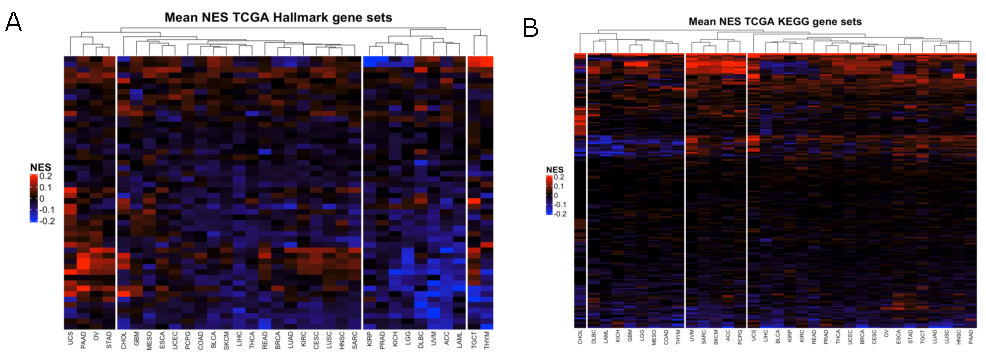
\includegraphics{~/Desktop/GitHub/2022-topic-02-team-02/09_figures/AppendixPanel6_Ebene 1.pdf}
  \caption{\textbf{Supplement: `GSEA` results for 33 tumor types} (A) Heatmap showing enrichment of hallmark gene sets in all tumor types (B) Heatmap showing enrichment of KEGG gene sets in all tumor types}
  \label{hmap}
\end{figure}

\begin{figure}[h]
 \begin{center}
   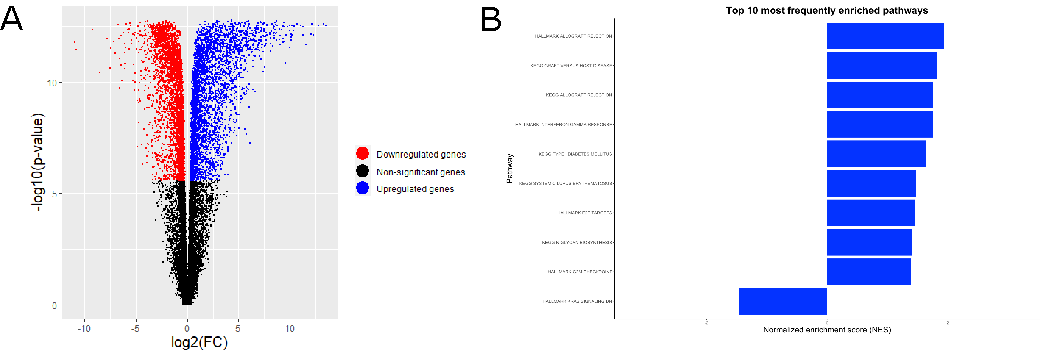
\includegraphics{~/Desktop/GitHub/2022-topic-02-team-02/09_figures/Appendix_Panel4_Ebene 1.pdf}
  \end{center}
  \caption{\textbf{Supplement: Identification of differences between healthy and tumorous tissue in KIRC } (A) Volcano plot showing differential gene expression between healthy and tumorous tissue (B) Top 10 most frequently enriched pathways}
  \label{volcanoap}
\end{figure}

\begin{figure}[h]
 \begin{center}
   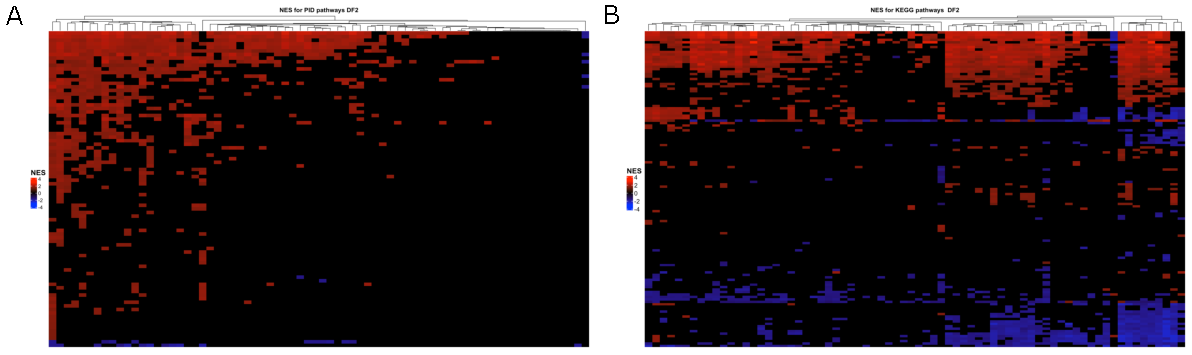
\includegraphics{~/Desktop/GitHub/2022-topic-02-team-02/09_figures/Appendix_tuktuktuk_Ebene 1.pdf}
  \end{center}
  \caption{\textbf{Supplement: GSEA results for PID and KEGG pathways in DF2 } (A) } (A) Heatmap showing ES for PID pathways (B) Heatmap showing ES for KEGG pathways
  \label{tuk}
\end{figure}

\pagebreak

\hypertarget{packages-1}{%
\section{Packages}\label{packages-1}}

\begin{longtable}[]{@{}lll@{}}
\caption{Packages used for analysis}\tabularnewline
\toprule
Package & Author & Application \\
\midrule
\endfirsthead
\toprule
Package & Author & Application \\
\midrule
\endhead
biomaRt & (Durinck \emph{et al.}, 2005) & biotype filtering \\
circlize & (Gu \emph{et al.}, 2014) & color scaling for heatmaps \\
ComplexHeatmap & (Gu \emph{et al.}, 2016) & heatmap plots \\
dplyr & (Wickham \emph{et al.}, 2022) & data transformation \\
factoextra & (Kassambara and Mundt, 2020) & visualization of kmeans
results \\
fgsea & (Korotkevich \emph{et al.}, 2019) & curration of pathway
activity matrix \\
ggdendro & (de Vries and Ripley, 2022) & hierarchical clustering \\
ggplot2 & (Wickham, 2016) & plots \\
ggpubr & (Kassambara, 2020) & r - optimization of heat map plots \\
grid & (R Core Team, 2022a) & creation of plot panels \\
msigdbr & (Dolgalev, 2022) & curration of pathways \\
reshape2 & (Wickham, 2007) & data preperation for ggplot \\
stats & (R Core Team, 2022b) & statistical testing \\
stringr & (Wickham, 2019) & text formatting \\
tidyverse & (Wickham \emph{et al.}, 2019) & data transformation \\
umap & (Konopka, 2022) & dimension reduction, visualisation of PCA
results \\
uwot & (Melville, 2021) & UMAP, dimension reduction \\
\bottomrule
\end{longtable}

\end{document}
